\chapter{Filtering methods}
\label{sec:filter}

In this chapter, I present various filtering methods for approximate string matching.
I consider two classes of filtering methods: those based on \emph{seeds} and those based on \emph{$q$-grams}.
Filters of the former class partition the pattern into \emph{non-overlapping} factors called seeds, while filters of the latter class consider all \emph{overlapping} substrings of the pattern having length $q$, the so-called $q$-grams.
Both classes include various combinatorial filtering methods of increasing specificity and complexity, always providing filtration schemes with guarantees on filtration sensitivity.

I consider the following seed filtering methods:
%\begin{inparaenum}[(i)]
\emph{exact seeds} \citep{Baeza1992},
\emph{approximate seeds} \citep{Myers1994,Navarro2000},
\emph{suffix filters} \citep{Kaerkkaeinen2007}.
%\end{inparaenum}
Exact seeds partition the pattern in $k+1$ non-overlapping seeds, to be searched exactly.
Approximate seeds increase specificity by factorizing the pattern in less than $k+1$ non-overlapping seeds, to be searched within a smaller distance threshold.
Suffix filters further generalize exact and approximate seeds and yield stronger index based filtration.

I consider the following $q$-gram filtering methods:
%\begin{inparaenum}[(i)]
\emph{contiguous $q$-grams} \citep{Jokinen1991},
\emph{gapped $q$-grams} \citep{Burkhardt2001},
\emph{multiple gapped $q$-grams} \citep{Kucherov2005}.
%\end{inparaenum}
Contiguous $q$-grams rely on a counting argument to filter out text regions containing less than a given threshold of $q$-gram occurrences.
Gapped $q$-grams introduce \emph{don't care positions} to lower the correlation between occurrences of consecutive $q$-grams.
Multiple gapped $q$-grams conjunct multiple patterns of don't care positions to further increase specificity.

It will become clear through this chapter that seed filters are more practical, flexible, straightforward to design and implement than $q$-gram filters.
All seed filters and contiguous $q$-grams provide full-sensitive filtration schemes for the $k$-differences problem, while (multiple) gapped $q$-grams only for $k$-mismatches.
The design of highly specific yet full-sensitive filtration schemes for $q$-gram filters is combinatorially hard, while it is quite straightforward for seed filters.
Also implementation-wise, $q$-gram filters are more involved than seeds filter.
In fact, seed filters lend themselves well to both online and offline variants of the problem, while $q$-gram filters are better suited for the online variant.
Finally, the experimental evaluation shows that seed filters outperform $q$-gram filters for most practical inputs.
For these reasons, I design the applications of chapters \ref{sec:masai} and \ref{sec:yara} around seed filtering methods.

%Problems of exact and approximate seeds filters are that: it is not evident which factorization yields optimal filtration, and they yield duplicate occurrences whenever errors are not distributed in the worst-case combination.
%The drawback is that the effort to implement them is slightly higher.

%In the following of this chapter I first present (multiple) gapped $q$-grams and problems associated with their design.
%Then I move to more practical approximate seeds, which I will adopt later in chapter~\ref{chap:map-eng}.
%Finally I discuss suffix filters and their practicality.

%Overall, through this chapter:
%\begin{itemize}
%\item I present a framework for the design of (multiple) gapped $q$-grams consisting of efficient exact and approximate solutions;
%\item I provide generic parallel implementations of filters based on exact and approximate seeds;
%\item I evaluate these filtration schemes in practice.
%\end{itemize}

% -----------------------------------------------------------------------------

\section{Exact seeds}
\label{sec:filtering:exact}

Filtration with exact seeds is one of the na\"ivest filtering methods for approximate string matching.
I first explain the underlying combinatorial principle, then I discuss implementation details and lastly give some insights on the efficiency of this method.

\subsection{Principle}

I consider the case of two arbitrary strings $x,y$ within edit distance $k$.
The generalization to $k$-differences is straightforward.

%If I partition \wlogs $y$ into $k+1$ non-overlapping seeds, then at least one seed will occur as a factor of $x$.
\begin{lemma}
\label{lemma:exact-seeds}
\citep{Baeza1992}
Let $x,y$ be two strings \st $d_E(x,y) = k$.
%If $y=y^1 y^2 \dots y^{k+1}$ then $x=ay^ib$ for some $a, b$.
If $y$ is partitioned \wlogs into $k+1$ non-overlapping seeds, then at least one seed occurs as a factor of $x$.
\end{lemma}
%\begin{proof}
%I proceed by induction on $k$.
%For $k=0$, the string $y$ is partitioned into one factor, $y$ itself.
%The condition $d_E(x,y) = 0$ implies $x=y$, which is true for $a=\epsilon$ and $b=\epsilon$.
%I suppose the case $k=j-1$ to be true, thus since $d_E(x,y) = j-1$ and $y=y^1 y^2 \dots y^{j}$ then $x=ay^ib$ for some $a, b$.
%I consider the case $k=j$. The $j$-th error can be in
%\begin{inparaenum}[(i)]
%\item\label{lemma:exact-seeds:prefix} $y^1\dots y^{i-1}$,
%\item\label{lemma:exact-seeds:infix} $y^i$, or
%\item\label{lemma:exact-seeds:suffix} $y^{i+1}\dots y^{j}$.
%\end{inparaenum}
%In case~\ref{lemma:exact-seeds:prefix} or~\ref{lemma:exact-seeds:suffix}, $x=ay^ib$ clearly holds.
%In case~\ref{lemma:exact-seeds:infix}, if I partition $y^i$ in two factors $y^{i'}$ and $y^{i''}$, then either $x=ay^{i'}b'$ or $x={a'}y^{i''}b$.
%\end{proof}
It is immediate to see that any edit distance error can cover at most one seed.
Therefore, at least one seed of $y$ will not be covered by any seed and hence occur as a factor of $x$.
Figure~\ref{fig:seeds-ext} shows an example.

\begin{figure}[h]
\begin{center}
\caption{Filtration with exact seeds.}
\label{fig:seeds-ext}
\begin{tikzpicture}[font=\normalsize]

\tikzstyle{n}=[inner sep=0pt, minimum size=10pt, align=center]
\tikzstyle{e}=[-latex, thin]
\tikzstyle{m}=[draw, shape=circle, clabel, pos=0.4, align=center, inner sep=0pt, minimum size=8pt, font=\tiny]
\tikzstyle{t}=[draw, shape=circle, clabel, pos=0.4, align=center, inner sep=0pt, minimum size=8pt, font=\tiny, fill=LightGray]
\tikzstyle{frame}=[draw, rectangle, thin, inner sep=0pt]
\tikzstyle{covered}=[draw, rectangle, thin, inner sep=0pt, fill=LightGray]
\tikzstyle{tape}=[fill=black]
\tikzstyle{strike}=[-, style=double, ultra thin, decorate, decoration=zigzag]
\tikzstyle{line}=[-, thin]
\tikzstyle{wave}=[-, thin, decorate, decoration={snake, segment length=2.5mm, amplitude=0.4mm}]


\newcommand{\transcript}[2]
{
    \foreach[count=\i] \r/\t/\g in {#2}
    {
    	\node[n] (read_\i) at (0.4*\i,0) {\r};
		\node[n] (genome_\i)  at (0.4*\i,-1) {\g};
		\ifthenelse{\equal{\t}{M}}
	    {
			\draw[e] (read_\i) -- (genome_\i) node[m] (transcript_\i) {\t};
		}
		{
			\draw[e] (read_\i) -- (genome_\i) node[t] (transcript_\i) {\t};
		}
    }
    
    \begin{pgfonlayer}{background} 
		\draw[tape] ([xshift=0.1cm, yshift=-0.01cm]transcript_1.north west) rectangle ([xshift=-0.1cm, yshift=0.01cm]transcript_#1.south east) ;
	\end{pgfonlayer}
}

\newcommand{\seed}[3]
{
	\ifthenelse{\equal{#3}{0}}
    {
%    	\draw[strike] (read_#1.west) -- (read_#2.east) ;

	    \begin{pgfonlayer}{background} 
    		\draw[covered] (read_#1.north west) rectangle (read_#2.south east) ;
		\end{pgfonlayer}
    }
           
	\node[frame] (read_rect) [transform shape, fit = (read_#1) (read_#2)] {};
}

\newcommand{\band}[1]
{
%	\node[frame] (genome_rect) [transform shape, fit = (genome_1) (genome_#1)] {};

	\draw[line] (genome_1.north west) -- (genome_#1.north east) ;
	\draw[line] (genome_1.south west) -- (genome_#1.south east) ;
	\draw[line] (genome_1.north west) -- (genome_1.south west) ;
	\draw[line] (genome_#1.north east) -- (genome_#1.south east) ;
}

\transcript{25}{G/M/G, C/M/C, T/M/T, N/R/A, T/M/T, G/M/G, G/D/$-$, G/M/G, C/M/C, A/M/A, T/M/T, T/M/T, A/R/G, T/M/T, G/M/G, G/M/G, C/M/C, $-$/I/C, C/M/C, A/M/A, T/M/T, T/M/T, T/M/T, T/R/A, T/M/T}
\band{25}

\node[left=0.25cm of read_1] {$x$} ;
\node[left=0.25cm of genome_1] {$y$} ;
\node[left=0.25cm of transcript_1] {$transcript$} ;

% (a) Exact seeds
% GCTN TGGG CATT ATGG C-CAT TTTT
% GCTA TG-G CATT GTGG CCCAT TTAT
%
\seed{1}{4}{0}
\seed{5}{8}{0}
\seed{9}{12}{1}
\seed{13}{16}{0}
\seed{17}{21}{0}
\seed{22}{25}{0}

% (b) Approximate seeds
% GCTNTGGG CATTATGG C-CATTTTT
% GCTATG-G CATTGTGG CCCATTTAT
%
%\seed{1}{8}{0}
%\seed{9}{16}{1}
%\seed{17}{25}{0}

\end{tikzpicture}
\end{center}
\end{figure}

This filtering method reduces the approximate search into multiple smaller exact searches.
It solves $k$-differences by partitioning the pattern into $k+1$ seeds, searching all seeds into the text, and verifying all their occurrences in the text.
As lemma~\ref{lemma:exact-seeds} is valid for \emph{any substring} of the text within distance $k$ from the pattern, this method finds all approximate occurrences of the pattern in the text.

%\subsection{Implementation}
%\subsubsection{Filtration step}
%Due to its simplicity, this filtering method lends itself to both online and offline implementations.
%In the online implementation, all seeds are preprocessed \eg in a  index.
%In the offline implementation, seeds are looked up in the text index.

%\subsubsection{Redundancy}
%
%Redundancy is a practical problem of seed filters.
%Whenever errors are not distributed according to a worst-case combination for lemma~\ref{lemma:exact-seeds}, more than one seed reports the same candidate location.
%For instance, if two errors fall in the same seed, then at least two seeds will occur exactly.
%
%In practice, redundancy can be avoided either before or after the verification step.
%In the first case, any diagonal in the implicit DP matrix identifies a distinct pattern occurrence to be verified only once.
%All candidate locations of a pattern have to be collected, then sorted by diagonal position and checked.
%Alternatively, if the verification algorithm is fast or the number of redundant candidate locations is low, it is more appealing to verify candidate locations directly.
%Any two pattern occurrences beginning or ending at the same location in the text are redundant.
%To avoid reporting duplicate occurrences, all pattern occurrences have to be collected, sorted and checked.
%
%How many redundant error configurations are produced by filtration with exact seeds?
%Here I consider the fraction of redundant error combinations, not the fraction of redundant candidate locations reported by the filter.
%For simplicity, I consider only combinations of exactly $k$ errors.
%Filtration has to cover all possible ways of distributing $k$ errors among $k+1$ seeds, that is $\binom{2k}{k}$ error combinations.
%However, a fixed seed covers all combinations where the seed itself contains no errors and all $k$ errors are distributed among the remaining $k$ seeds, \ie $\binom{2k-1}{k}$ error combinations.
%Thus the fraction of error combinations covered by filtration with exact seeds over the minimal ones is
%\begin{equation}
%\frac{(k+1)\binom{2k-1}{k}}{\binom{2k}{k}} = \frac{k+1}{2}.
%\end{equation}
%For instance, when $k=5$, filtration with exact seeds covers 3 times more combinations than required.

\subsection{Efficiency}
\label{sec:filtering:exact:efficiency}

%Efficiency depends number of verifications - filtration time is negligible.

How many verifications are triggered by filtration with exact seeds?
It is straightforward to derive the expected number of verifications under the assumption of the text being generated according to the uniform Bernoulli model.
The emission probability of any symbol in $\Sigma$ is $p = \frac{1}{\sigma}$ and under \iid assumptions the emission (and occurrence) probability of any word of length $q$ is simply
\begin{eqnarray}
\text{Pr}(H > 0) = \frac{1}{\sigma^q}
\end{eqnarray}
thus the expected number of occurrences of a seed of length $q$ in a text of length $n$ is
\begin{eqnarray}
E[H] = \sum_{i=1}^{n-q+1}{\text{Pr}(H > 0)} = \frac{n - q + 1}{\sigma^q} \leq \frac{n}{\sigma^q}.
\end{eqnarray}

Lemma~\ref{lemma:exact-seeds} requires to partition the pattern into $k+1$ seeds but leaves the freedom to choose their length.
This leads to the problem of finding an optimal pattern partitioning to minimize the expected number of verifications.
I fix\footnote{For simplicity I ignore that some seed could have length $\left \lceil \frac{m}{k+1} \right \rceil$.} the length of all seeds to be
\begin{eqnarray}
\label{eq:seed-len}
q=\left \lfloor \frac{m}{k+1} \right \rfloor
\end{eqnarray}
to minimize the expected number of occurrences of any seed.
Under these conditions, the expected number of verifications produced by filtration with exact seeds is
\begin{eqnarray}
E[V] = E[H] \cdot (k + 1) < \frac{n (k + 1)}{\sigma^q}.
\end{eqnarray}
Nonetheless, inputs of practical interest like genomes and natural texts do not fit well the uniform Bernoulli model.
On those texts, uniform seed length often leads to suboptimal filtration.

%\subsubsection{Expected sublinearity}
%I now turn to the effect of the error rate on the runtime of the resulting $k$-differences algorithm.
%For which error rate the resulting algorithm is expected to have \emph{sublinear} runtime?
%\citeauthor{Gusfield1997} gives a rough estimate to this question.
%If the classic $\Oh(m^2)$ DP algorithm of section~\ref{sub:introonline} is adopted to verify candidate locations, the expected runtime must be
%\begin{eqnarray}
%E[V] \cdot m^2 < cn
%\end{eqnarray}
%for some constant $c$.
%Substituting $E[V]$ and solving for $q$ yields
%\begin{eqnarray}
%q > \log_{\sigma}{\frac{m^3}{c}}
%\end{eqnarray}
%and since $q$ in equation~\ref{eq:seed-len} is a function of $m$ and $k$, it follows that
%\begin{eqnarray}
%\epsilon = \frac{k}{m} < \frac{m}{\log_{\sigma}{m}}
%\end{eqnarray}
%is the error rate for which this $k$-differences algorithm has expected sublinear runtime.

% -----------------------------------------------------------------------------

\section{Approximate seeds}
\label{sec:seeds-apx}

The simple analysis of section~\ref{sec:filtering:exact:efficiency} shows that filtration specificity is strongly correlated to the seed length.
Therefore, the crux of designing a stronger filter lies into increasing the seed length while maintaining the full-sensitivity constrains.
\citeauthor{Myers1994}, subsequently followed by \citeauthor{Navarro2000}, proposed \emph{approximate seeds} as a practical and effective generalization of exact seeds, yielding stronger filters for $k$-differences.
The key idea of approximate seeds is to reduce the approximate search into smaller approximate searches, as opposed to exact seeds that reduce the approximate search into smaller exact searches.

\subsection{Principle}

Again, I start by considering two arbitrary strings $x,y$ within edit distance $k$.
The result then holds for any substring of the text within distance $k$ from the pattern.
\begin{lemma}
\label{lemma:apx-seeds}
\citep{Myers1994,Navarro2000}
Let $x,y$ be two strings \st $d_E(x,y) = k$.
If $y$ is partitioned \wlogs into $s$ non-overlapping seeds \st $1 \leq s \leq k+1$, then at least one seed occurs as a factor of $x$ within distance $\lfloor k/s \rfloor$.
\end{lemma}
To prove full-sensitivity it suffices to see that, if none of the seeds occurs within its assigned distance, the total distance must be greater than $s \cdot \lfloor k/s \rfloor = k$.
Figure~\ref{fig:seeds-apx} illustrates.

\begin{figure}[h]
\begin{center}
\caption[Filtration with approximate seeds]{Filtration with approximate seeds.}
\label{fig:seeds-apx}
\begin{tikzpicture}[font=\normalsize\sffamily]

\transcript{25}{G/M/G, C/M/C, T/M/T, N/R/A, T/M/T, G/M/G, G/D/$-$, G/M/G, C/M/C, A/M/A, T/M/T, T/M/T, A/R/G, T/M/T, G/M/G, G/M/G, C/M/C, $-$/I/C, C/M/C, A/M/A, T/M/T, T/M/T, T/M/T, T/R/A, T/M/T}{1}
\band{25}
\seed{1}{25}{1}

\node[left=0.25cm of read_1] {$p$} ;
\node[left=0.25cm of genome_1] {$t$} ;

\qgrama{1}{$\#$, $\#$, $\#$, $\#$, $\#$, $\#$, $\#$, $\#$}{1}{8}
\qgrama{9}{$\#$, $\#$, $\#$, $\#$, $\#$, $\#$, $\#$, $\#$}{1}{8}
\qgramai{17}{$\#$, $ $, $\#$, $\#$, $\#$, $\#$, $\#$, $\#$, $\#$}{1}{8}

\draw[strike] (qgram_1_4.north) -- (qgram_1_4.south) ;
\draw[strike] (qgram_1_7.north) -- (qgram_1_7.south) ;
\draw[strike] (qgram_9_5.center)  -- (qgram_9_5.south) ;
\draw[strike] (qgram_17_8.north) -- (qgram_17_8.south) ;

\end{tikzpicture}
\end{center}
\end{figure}

Lemma \ref{lemma:apx-seeds} assigns the same distance threshold to all seeds, yet this is not obligatory.
I give here a more general definition of approximate seeds.

\begin{lemma}
\label{lemma:apx-seeds-var}
Let $x,y$ be two strings \st $d_E(x,y) = k$.
Partition $y$ into $s$ non-overlapping seeds $y^1, y^2, \dots, y^s$.
Assign an arbitrary distance threshold $k_i$ to each seed $y^i$, satisfying the following constraint:
\begin{equation}
s + \sum_{i=1}^{s}{k_i} > k.
\end{equation}
Then at least one seed occurs as a factor of $x$ within distance $k_i$.
\end{lemma}

%\subsection{Implementation}
%Online/Offline.

\subsection{Parameterization}

Approximate seeds provide filtration schemes of increasing specificity.
The fastest but weakest scheme is given by $s=k+1$, while the most specific filtration scheme is obtained for $s=1$ \ie perfect filtration without any verification step.
Alternatively, filtration specificity is controlled by acting on the minimum seed length $q$.
Fixing $q$ yields $s = \lfloor m/q \rfloor$, or vice versa, fixing the number of seeds $s$ gives $q =\lfloor m/s \rfloor$.
As expected, filtration specificity increases with seed length.

How to choose a good filtration scheme in practice?
\citeauthor{Myers1994}, \citeauthor{Navarro2000} carried out involved analysis to estimate the optimal parameterization. \citeauthor{Navarro2000} find out that a number of seeds of $\Theta(\frac{m}{\log_{\sigma}{n}})$ yields an overall time complexity sublinear for an error rate $\epsilon < 1 - \frac{e}{\sqrt{\sigma}}$.
\citeauthor{Myers1994} reports an analogous sublinear time when $q=\Theta(\log_{\sigma}{n})$ is the seed length.
Yet, these results do not necessarily translate into optimal filtration schemes in practice.
The parameterization depends on the full-text index, the verification algorithm, the statistical properties of the text.
Missing the optimal number of seeds by one often results in a runtime penalty of an order of magnitude.

Having established the number of seeds, or their length, thresholds have to be assigned.
Lemma \ref{lemma:apx-seeds-var} allows to assign arbitrary distance thresholds.
In practice, it is convenient to distribute distance thresholds evenly, as seeds with the highest threshold dominate the overall filtration time.
The most strict threshold assignment is to give distance $\lfloor k/s \rfloor$ to $(k \bmod{s}) + 1$ seeds and distance $\lfloor k/s \rfloor - 1$ to the remaining seeds \citep{Siragusa2013}.

% -----------------------------------------------------------------------------

%\section{Suffix filters}

% -----------------------------------------------------------------------------

\section{Contiguous $q$-grams}
\label{sec:filtering:qgrams-ext}

$q$-Gram filters rely on counting arguments to filter out text regions containing less than a given threshold of $q$-gram occurrences.
The first $q$-gram counting filter has been proposed in \citep{Jokinen1991}.
More general filters have been proposed and implemented in \emph{QUASAR} \citep{Burkhardt1999}, \emph{SWIFT} \citep{Rasmussen2006}, \emph{STELLAR} \citep{Kehr2011}.

\subsection{Principle}

The counting argument of contiguous $q$-gram filters is based on the so-called \emph{$q$-gram similarity measure} $\tau_q : \Sigma^{*} \times \Sigma^{*} \rightarrow \N_0$, defined as the number of substrings of length $q$ common to two given strings.
The following lemma relates $q$-gram similarity to edit distance.
It gives a lower bound on the $q$-gram similarity $\tau_q(x,y)$ of any two strings $x,y$ within edit distance $k$.
As for seed filters, the result then easily translates to $k$-differences.

\begin{lemma}[The $q$-gram lemma] \citep{Jokinen1991}
\label{lemma:qgrams}
Let $x,y$ be two strings \st $d_E(x,y) = k$, and assume \wlogs $|x| \leq |y|$ and $|x| = m$. Then $x$ and $y$ have $q$-gram similarity $\tau_q(m,k) \geq m - q + 1 - kq$.
\end{lemma}
The first part of the threshold function $\tau$ counts the number of $q$-grams of $x$ (\ie $m - q + 1$), while the second part counts how many $q$-grams can be covered by $k$ errors ($kq$, \ie at most $q$ per error).
The threshold function $\tau$ depends only on parameters $q,m,k$ and not on the specific $q$-grams.
Figure~\ref{fig:qgrams-ext} illustrates.

\begin{figure}[h]
\begin{center}
\caption[Filtration with contiguous $q$-grams] {Filtration with contiguous $q$-grams.}
\label{fig:qgrams-ext}
\begin{tikzpicture}[font=\normalsize\sffamily]

\transcript{25}{G/M/G, C/M/C, T/M/T, N/R/A, T/M/T, G/M/G, G/M/G, G/D/$-$, C/M/C, A/M/A, T/M/T, A/R/G, T/M/T, T/M/T, G/M/G, A/R/G, G/M/C, C/M/C, C/M/C, G/R/A, T/M/T, T/M/T, T/M/T, A/M/A, T/M/T}{4}
\band{25}
\seed{1}{25}{1}

\node[left=0.25cm of read_1] {$\Pattern$} ;
\node[left=0.25cm of genome_1] {$\Text$} ;

% Unaffected q-grams ###-#
\foreach \x in {21,22}
{
	\pgfmathtruncatemacro{\y}{1+Mod(\x-1,4)}
	\qgram{\x}{$\#$, $\#$, $\#$, $\#$}{\y}{1}
}

% Covered q-grams ###-#
\foreach \x in {1,...,20}
{
	\pgfmathtruncatemacro{\y}{1+Mod(\x-1,4)}
	\qgram{\x}{$\#$, $\#$, $\#$, $\#$}{\y}{0}
}

% Strikes over covered q-grams
\foreach \x in {1,...,20}
{
	\pgfmathtruncatemacro{\y}{4-Mod(\x-1,4)}
	\draw[strike] (qgram_\x_\y.north) -- (qgram_\x_\y.south) ;
}

\end{tikzpicture}
\end{center}
\end{figure}

%\subsection{Implementation}
\subsection{Bucketing}

This filtering method requires \emph{bucketing} the text in windows to enforce the counting argument of lemma \ref{lemma:qgrams}.
Buckets are obtained by subdividing the implicit DP matrix in parallelograms and projecting them on the text.
Figure \ref{fig:swift} illustrates this concept: any approximate occurrence of the pattern in the text spans at most $k$ diagonals and is thus enclosed inside a parallelogram of width $k+1$ \citep{Rasmussen2006}.
Hence the projection of any text bucket has length $2k + 1$ and any occurrence has length between $m - k$ and $m + k$.
The implementations described in \citep{Rasmussen2006, Kehr2011, Weese2009} use more efficient bucketing strategies with larger, overlapping parallelograms.

\begin{figure}[h]
\begin{center}
\caption[Parallelogram buckets] {Parallelogram buckets. Picture from \citep{Weese2009}.}
\label{fig:swift}
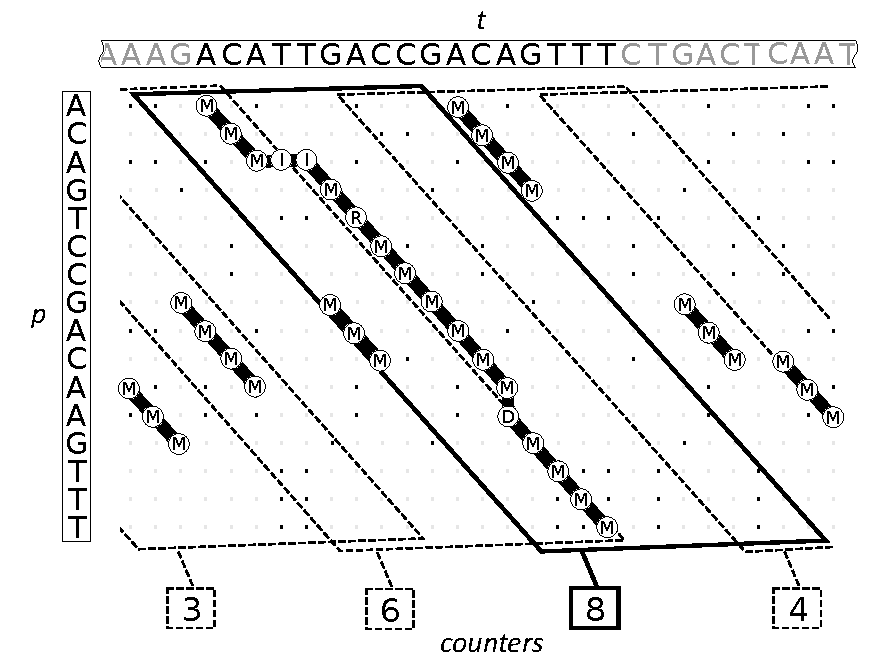
\includegraphics[scale=0.75]{figures/swift.pdf}
\end{center}
\end{figure}

This method lends itself to work in a multiple online fashion rather than offline.
The filtration stage scans the text and counts how many $q$-grams of the pattern fall into each bucket.
The verification stage then verifies only parallelograms exceeding threshold $\tau_q(m,k)$.
As long as the filter scans the text, such implementation remembers only buckets covering the patterns' lengths.
To speed up the filtration phase, an index of the text could be used to count the $q$-gram.
However, this implementation would require more memory, both to keep the text index in memory and to bucket the whole text.

\subsection{Parameterization}

Which is the biggest $q$-gram length yielding lossless filtration given $m$ and $k$?
In order to satisfy lemma~\ref{lemma:qgrams}, the $q$-gram threshold must be greater than zero, \ie it must hold $\tau_q(m,k) \geq 1$.
Thus, by substituting $\tau$, it follows that the $q$-gram length must be $q \leq \left \lfloor \frac{m}{k+1} \right \rfloor$, analogously to equation~\ref{eq:seed-len} of seed filters.
%However, a threshold of 1 does not make filtration very specific.

% -----------------------------------------------------------------------------

\section{Gapped $q$-grams}
\label{sec:filtering:qgrams-gapped}

The idea of \emph{gapped $q$-grams} is to lower the correlation between consecutive $q$-grams.
The occurrence of any contiguous $q$-gram is strongly correlated to the occurrences of its preceding and following $q$-grams.
One single edit distance error affects a cluster of $q$ consecutive $q$-grams, as evidenced by the $q$-gram lemma~\ref{lemma:qgrams}.
Gapped $q$-grams skip characters at fixed positions by defining patterns of \emph{don't care positions}.
Such don't care positions are immune to mismatches but not to insertions and deletions.
Hence, this generalization of contiguous $q$-grams is useful to solve $k$-mismatches but not $k$-differences.
%Filtration specificity increases either by raising the filtering threshold or the $q$-gram length, in either cases preserving full-sensitivity.

Gapped $q$-grams rely on a generalization of the $q$-gram similarity measure (section~\ref{sec:filtering:qgrams-ext}) to \emph{subsequences}.
A subsequence is a non-contiguous sequence of symbols of a given string.
Hence, instead of substrings, filtration with gapped $q$-grams counts the number of subsequences of length $q$ common to two strings, whose positions are taken from a fixed set $Q$.
The formal definition of gapped $q$-gram follows.

\begin{definition}
A $Q$-gram is a finite sequence $Q$ of natural numbers starting with the unit element, \ie $Q \subset \N$ and $1 \in Q$.
The cardinality $|Q|$ is called the \emph{weight} of $Q$ and denoted as $w(Q)$.
The maximum element of $Q$ is named \emph{span} and indicated by $s(Q)$.
\end{definition}
%In literature, $Q$-grams are visualized as words over the alphabet $\{1,*\}$ or $\{\#,-\}$.
%I adopt the former notation and represent the $Q$-gram by the word $w \in \{1,*\}^{s(Q)}$ such that $w_j=1$ iff $j \in Q$.

\begin{figure}[h]
\begin{center}
\caption[Filtration with gapped $q$-grams]{Filtration with gapped $q$-grams.}
\label{fig:qgrams-gapped}
\begin{tikzpicture}[font=\normalsize\sffamily]

\transcript{25}{G/1/G, C/1/C, T/1/T, T/1/T, N/0/A, G/1/G, T/1/T, G/1/G, C/1/C, G/0/A, T/1/T, A/1/A, T/1/T, T/1/T, A/0/G, A/1/A, G/1/C, C/1/C, C/1/C, G/0/A, T/1/T, T/1/T, A/0/T, A/1/A, T/1/T}{5}
\band{25}
\seed{1}{25}{1}

\node[left=0.25cm of read_1] {$\Pattern$} ;
\node[left=0.25cm of genome_1] {$\Text$} ;

% Unaffected q-grams ###-#
\foreach \x in {4,9,14}
{
	\pgfmathtruncatemacro{\y}{1+Mod(\x-1,5)}
	\qgramg{\x}{$\#$, $ $, $\#$, $\#$, $\#$}{\y}{1}
}

% Covered q-grams ###-#
\foreach \x in {1,2,3,5,6,7,8,10,11,12,13,15,16,17,18,19,20,21}
{
	\pgfmathtruncatemacro{\y}{1+Mod(\x-1,5)}
	\qgramg{\x}{$\#$, $ $, $\#$, $\#$, $\#$}{\y}{0}
}

% Strikes over covered q-grams
\foreach \x in {1,2,3,5,6,7,8,10,11,12,13,15,16,17,18,20}
{
	\pgfmathtruncatemacro{\y}{5-Mod(\x-1,5)}
	\draw[strike] (qgram_\x_\y.north) -- (qgram_\x_\y.south) ;
}
\draw[strike] (qgram_21_3.north) -- (qgram_21_3.south) ;
\draw[strike] (qgram_20_4.north) -- (qgram_20_4.south) ;
\draw[strike] (qgram_19_5.north) -- (qgram_19_5.south) ;

\end{tikzpicture}
\end{center}
\end{figure}

Figure~\ref{fig:qgrams-gapped} shows an example of $Q$-gram.
As in the $q$-gram lemma, the threshold depends only on $Q$ and parameters $m,k$.
Indeed, the pattern of occurring $q$-grams does not depend on the text or pattern sequences but only on their transcript, \ie on the mismatch positions.
As mismatches do not affect don't care positions, any gapped $Q$-gram potentially yields a higher threshold than the contiguous $q$-gram of the same weight.
Unfortunately, the $q$-gram lemma (\ref{lemma:exact-qgrams}) does not give anymore a tight threshold, but only a lower bound.

Gapped $q$-grams raise hard combinatorial questions.
\begin{inparaenum}[(i)]
\item \label{enum:qgram-non-detection} Does a given gapped $q$-gram yield a full-sensitive filter for $k$-mismatches? If so, either
\item \label{enum:qgram-threshold} which is the maximum $q$-gram threshold $t$ that guarantees full-sensitivity? Or alternatively,
\item \label{enum:qgram-error} which is the maximum error $k$ for which full-sensitivity is guaranteed?
If the answer to question~\ref{enum:qgram-nd} is negative and the filter is lossy,
\item \label{enum:qgram-fn} how many false negatives the filter discards?
Considering filtration efficiency,
\item \label{enum:qgram-fp} how many false positives the filter produces?
%If the weight is taken as a simplified criterion predicting filtration efficiency, 
%\item \label{enum:qgram-weight} which is the maximum weight lossless shape?
\end{inparaenum}

Question~\ref{enum:qgram-threshold} has been first considered in \citep{Burkhardt2001,Kucherov2005},
the more general questions~\ref{enum:qgram-non-detection} has been introduced in \citep{Nicolas2005}, while I consider here for the first time questions \ref{enum:qgram-error}-\ref{enum:qgram-fp}.
With the aim of elucidating these questions, I first introduce simple characteristic functions to formally define transcripts detected by gapped $q$-grams.
Afterwards, I recapitulate known results for questions \ref{enum:qgram-non-detection}-\ref{enum:qgram-fp} and present new exact and approximate solutions.

\subsection{Characteristic functions}

Consider an arbitrary transcript $\sigma$ as a $m$-dimensional vector over $\Bo$, where $|\sigma|_0$ indicates the Hamming distance of the transcript.
Let $\Bo^m_k \subset \Bo^m$ be the set containing all transcripts $\sigma$ such that $|\sigma|_0 = k$.

\begin{definition}
A $Q$-gram \emph{occurs} at position $i$ in a similarity $\sigma$ iff $\forall j \in Q$ $\sigma_{i+j}=1$.
Fixed a $Q$-gram threshold $t$, the $Q$-gram detects $\sigma$ iff it occurs at least $t$ times in $\sigma$.
\end{definition}

\subsubsection{Boolean functions}

Let $T_{Q}^{m}: \Bo^m \rightarrow \Bo$ denote a \emph{boolean function} such that $T_{Q}^{m}(\sigma)$ is true iff the $Q$-gram occurs at least one time in a similarity $\sigma$ of length $m$.
In general, $(Q,t)$ detects $\sigma$ iff $\sigma$ satisfies at least $t$ clauses of $T_{Q}^{m}$.
I define such boolean function as the disjunction
\begin{equation}
\label{eq:qgram-bool}
T_{Q}^{m}(\sigma) = \bigvee_{i=1}^{m-s(Q)+1} \bigwedge_{j \in Q} \sigma_{i+j}
\end{equation}
where each \emph{clause} of $T_{Q}^{m}$ represents a single possible occurrence of $Q$ in $\sigma$.
%The seed boolean function $T_{Q}^{m}$ describes the computation performed by the seed automaton $A_Q$ on all similarities of length $m$.
I define an analogous boolean function for a $Q$-gram family $F$ as the disjunction
\begin{equation}
\label{eq:family-bool}
T_{F}^{m}(\sigma) = \bigvee_{Q_i \in F} T_{Q_i}^{m}(\sigma)
\end{equation}
By definition, $T_{Q}^{m}$ and $T_{F}^{m}$ are \emph{monotone nondecreasing} boolean functions in \emph{disjunctive normal form} (\emph{DNF}).
Since all monotone boolean functions in DNF are minimal, $T_{Q}^{m}$ and $T_{F}^{m}$ are \emph{minimal}.

\subsubsection{Pseudo-boolean functions}

Let the function $t_{Q}^{m}: \Bo^m \rightarrow \N_0$ be the boolean function $T_{Q}^{m}$ acting on $\N_0$.
I define such \emph{pseudo-boolean function} as
\begin{equation}
\label{eq:qgram-pseudo}
t_{Q}^{m}(\sigma) = \sum_{i=1}^{m-s(Q)+1} \prod_{j \in Q}\sigma_{i+j}
\end{equation}
Here $t_{Q}^{m}(\sigma)$ counts how many times a $Q$-gram occurs in a similarity $\sigma$ of length $m$.
It is useful to define the complementary function $\bar{t}_{Q}^{m}$, counting how many times a $Q$-gram does not occur in a similarity $\sigma$, as
\begin{equation}
\label{eq:qgram-pseudoneg}
\bar{t}_{Q}^{m}(\sigma) = m - s(Q) + 1 - t_{Q}^{m}(\sigma)
\end{equation}
Analogously, I define a pseudo-boolean function for a $Q$-gram family $F$
\begin{equation}
\label{eq:family-pseudo}
t_{F}^{m}(\sigma) = \sum_{Q_i \in F} t_{Q_i}^{m}(\sigma)
\end{equation}
along with its complementary function
\begin{equation}
\label{eq:family-pseudoneg}
\bar{t}_{F}^{m}(\sigma) = \sum_{Q_i \in F}{(m - s(Q_i) + 1)} - t_{F}^{m}(\sigma)
\end{equation}

The above functions expose important properties which let me devise approximate solutions.
\emph{Nondecreasing monotonicity} of functions $t_{Q}^{m}$ and $t_{F}^{m}$ follow from nondecreasing monotonicity of their boolean counterparts $T_{Q}^{m}$ and $T_{F}^{m}$. Consequently $\bar{t}_{Q}^{m}$ and $\bar{t}_{F}^{m}$ are \emph{monotone nonincreasing}.
From definition~\ref{eq:supermodularity}, function $t_{Q}^{m}$ is \emph{supermodular}, thus it follows that $\bar{t}_{Q}^{m}$ is \emph{submodular}.
Since super and submodular functions are closed under non-negative linear combination, functions $t_{F}^{m}$ and $\bar{t}_{F}^{m}$ are respectively super and submodular.

\subsection{Full-sensitivity}

\textsc{Non Detection}~\citep{Nicolas2005}. Does a given $Q$-gram yield a full-sensitive filter for $k$-mismatches?

\subsubsection{Problem definition}

\paragraph{}
\begin{tabular}{rl}
{\bf Instance}	&	A $Q$-gram, two integers $m,k$ with $0 < k < m$. \\
{\bf Question}	&	Does it exist a similarity $\sigma \in \Bo^{m}_{k}$ such that $T_{Q}^{m}(\sigma)$ is false? \\
\end{tabular}
\\

\subsubsection{Hardness results}

\textsc{Non Detection} is \emph{strongly} NP-complete \citep{Nicolas2005}.
\citeauthor{Nicolas2005} introduce an intermediate problem, called \textsc{Soapy Set Cover}. They reduce \textsc{Exact Cover by 3-Sets} to \textsc{Soapy Set Cover} and \textsc{Soapy Set Cover} to \textsc{Non Detection}.
Strong NP-completeness implies that no \emph{FPTAS} nor any \emph{pseudo-polynomial} algorithm for it exist, under the assumption that $P \neq NP$.


\subsection{Optimal threshold}

Which is the highest $Q$-gram threshold $t$ that guarantees full-sensitivity?
This problem has been introduced in \citep{Burkhardt2001}. %and generalized in \citep{Kucherov2005}.

\subsubsection{Problem definition}

\paragraph{}
\begin{tabular}{rl}
{\bf Instance}	&	A $Q$-gram, two integers $m,k$ such that $0 < k < m$.\\
{\bf Solution}	&	The largest integer $t^*$ such that \textsc{Non Detection} for $(Q,t^*),m,k$ answers \emph{no}.\\
\end{tabular}
\\

Recalling $Q$-gram pseudo-boolean functions \ref{eq:qgram-pseudo}, I can define the optimal threshold problem as the minimization of a supermodular function subject to linear constraints
\begin{equation}
\begin{array}{ll}
\min & t_{Q}^{m} (\sigma)			\\
w.r.t.								\\
& \sigma \in \Bo^m_k				\\
\end{array}
\end{equation}

\subsubsection{Exact DP solution}

Optimal threshold is fixed-parameter tractable (FPT) in the span of the $q$-gram shape.
\citeauthor{Burkhardt2001} give a DP algorithm computing the optimal threshold in time $O(m \cdot k \cdot 2^{s(Q)})$ \citep{Burkhardt2001}.
\citeauthor{Kucherov2005} give an extension for $Q$-gram families \citep{Kucherov2005}.

%All possible assignments, \ie $\Bo^s(Q)$, for the first clause $\bigwedge_{j \in Q}{\sigma_j}$ of the boolean function $T_{Q}^{m}$ are considered and all satisfying assignments for it, \ie $\phi(Q)$, are computed.
%Clause $Q_2$ is considered next...

\subsubsection{Exact ILP solution}

I reduce this problem to \emph{maximum coverage} \citep{Vazirani2001} and solve it with the following ILP
\begin{equation}
\begin{array}{ll}
\max & |c|_1					\\
w.r.t.							\\
& \sigma \in \Bo^m_k			\\
& c \in \Bo^{m - s(Q) + 1}		\\
& \sigma_i \geq c_j				\\
\end{array}
\end{equation}
where variable $c_j$ indicates the truthfulness of the $j$-th clause in $T_{Q}^{m}$.
The optimal threshold $t^* = |c^*|_1$ is then obtained from the ILP solution $c^*$.

\subsubsection{APX solution}

I reduce the complementary optimal threshold problem to the maximization of a submodular function subject to linear constraints
\begin{equation}
\begin{array}{ll}
\max & \bar{t}_{Q}^{m}(\sigma)		\\
w.r.t.								\\
& \sigma \in \bar{\Bo}^m_k			\\
\end{array}
\end{equation}
where the complementary optimal threshold is $\bar{t}^* = m - s(Q) + 1 - t^*$.

I compute an approximate solution via deepest descent.
My greedy algorithm for complementary \textsc{Optimal Threshold} has an APX-ratio of $1 + 1/e$ \citep{Vazirani2001}.
The same \emph{absolute error} applies to \textsc{Optimal Threshold}.

\subsection{Maximum error}

Which is the maximum error $k^*$ for which full-sensitivity is guaranteed?

\subsubsection{Problem definition}

\paragraph{}
\begin{tabular}{rl}
{\bf Instance}	&	A $Q$-gram, an integer $m > 0$.\\
{\bf Solution}	&	The largest integer $k^*$ such that \textsc{Non Detection} for $Q,m,k^*$ answers \emph{no}.\\
\end{tabular}
\\

Recalling pseudo-boolean functions \ref{eq:qgram-pseudo}, I define this problem as the minimization of a linear function subject to submodular constraints
\begin{equation}
\begin{array}{ll}
\min & |\sigma|_1			\\
w.r.t.								\\
& \sigma \in \Bo^m					\\
& \bar{t}_{Q}^{m}(\sigma) \leq 0	\\
\end{array}
\end{equation}

\subsubsection{ILP solution}

I reduce the problem to \textsc{Minimum Set Cover} \citep{Vazirani2001}, solve it with the following ILP
\begin{equation}
\begin{array}{ll}
\min & |\sigma|_1	\\
w.r.t.				\\
& \sigma \in \Bo^m	\\
& b \in \Bo^{m-s(Q)+1}\\
& A\sigma \geq b	\\
\end{array}
\end{equation}
where the value $A_{ij}$ of the coefficient matrix $A$ is defined as
\begin{equation}
A_{ij} = 
\left\{
	\begin{array}{ll}
		1  & \mbox{if } i-j+1 \in Q		\\
		0  & \mbox{if } i-j+1 \notin Q	\\
	\end{array}
\right.
\end{equation}
and find the maximum error for which full-sensitivity is guaranteed as $k^* = |\bar{\sigma}^*|_1$ given the solution $\sigma^*$ to the ILP.

Contiguous $q$-grams provide an interesting special case of this ILP.
If $A$ has the \emph{consecutive ones property}, it is \emph{totally unimodular}.
The \emph{polytope} defined by a totally unimodular coefficient matrix is \emph{integral}.
Hence the optimal solution of the relaxed LP is also the optimal solution of the original ILP.


\subsubsection{APX solution}

Again, I compute an approximate solution via deepest descent.
APX-ratio of $H_{w(Q)}$ \citep{Vazirani2001}.


\subsection{Specificity}

How many false positives the filter produces?

\subsubsection{Problem definition}

\paragraph{}
\begin{tabular}{rl}
{\bf Instance}	&	A $Q$-gram, two integers $m,k$ such that $0 < k < m$.\\
{\bf Solution}	&	The number of false positives produced by the $Q$-gram.\\
\end{tabular}
\\

False positives are true points of the boolean function \ref{eq:qgram-bool} which have weight inferior to $m-k$ and satisfy more than $t$ clauses of $T_{Q^t}^{m}$.
Hence, I define the function $\text{FP}_{k}^{m}$ counting the number of false positives of filter $(Q,t)$ in instance $(m,k)$ as
\begin{equation}
\text{FP}_{k}^{m}(Q,t) = \sum_{\sigma \in {\bar{\Bo}^{m}_{k}}} T_{Q,t}^{m}(\sigma)
\end{equation}

\subsubsection{FPRAS solution}

I reduce counting false positives to counting the number of true assignments of a boolean function in DNF.
\citeauthor{Karp1989} introduce a \emph{FPRAS} approximating the number of true points of a DNF.
This problem can be approximated via importance sampling \citep{Vazirani2001}.

%\subsection{Sensitivity and specificity}
%and \ref{enum:qgram-fn}.

%\subsection{Optimal gapped $q$-grams}
%
%Introduced in \citep{Nicolas2005}.
%
%\subsubsection{Problem definition}
%
%\paragraph{}
%\begin{tabular}{rl}
%{\bf Instance}	&	A finite set $S$ of similarities.\\
%{\bf Solution}	&	A $Q$-gram that detects all similarities of $S$.\\
%{\bf Measure}	&	The weight $w(Q)$ of the $Q$-gram.\\
%\end{tabular}
%\\
%
%Given a set of similarities, find the $Q$-gram of maximum weight detecting all similarities.
%This applies to the DNA Homology Search Framework as well.
%%The MWLS is not the optimal seed for approximate string matching filtration nor for sequence homology filtration.
%%On one hand the weight is just an estimator of sensibility regardless of threshold, on the other hand filtration speed decreases with increasing weight.
%
%\subsubsection{Hardness and inapproximability results}
%
%Nicolas et al. \citep{Nicolas2005} perform an approximation preserving reduction from \textsc{Maximum Independent Set}.
%MWLS is NP-hard and APX-hard within $(|S|)^{0.25 - \epsilon}$ unless $P = NP$.
%If $S = \Bo^{m}_{k}$, $|S| = \binom{m}{k}$.
%
%\subsubsection{Branch-and-bound search}
%
%Burkhardt et al. \citep{Burkhardt2001} bounding criterion. If $Q_1 \subseteq Q_2$, then $t_{Q_2}(m,k) \leq t_{Q_1}(m,k)$.
%Such bounding criterion allows to discard parts of the search space which do not solve the considered $(m,k)$ instance.
%%The search space of seed families is more dense than the search space of single seeds (i.e. almost all seed families solve a give Non Detection instance). Thus search space pruning would not be as effective.

% -----------------------------------------------------------------------------

%\section{Verification methods}
%\label{sec:verification}
%\section{Myers' bit-vector algorithm}
%\subsection{Banded Myers' bit-vector algorithm}
%\subsection{Increased bit-parallelism using SIMD instructions}
